\section{Basic Tutorials 2}

%%%%%%%%%%%%%
\subsection{Filters}

%% Break
\begin{frame}{Basic Tutorial 2}
\fontsize{36pt}{36pt}\selectfont
\center
\begin{center}
Basic Tutorial 2
\end{center}
\end{frame}

\begin{frame}{Wrapped Languages}
\fontsize{36pt}{36pt}\selectfont
\center
\begin{center}
Wrapped Languages
\end{center}
\end{frame}

\begin{frame}[fragile]
\frametitle{Wrapping Process}
\begin{center}
  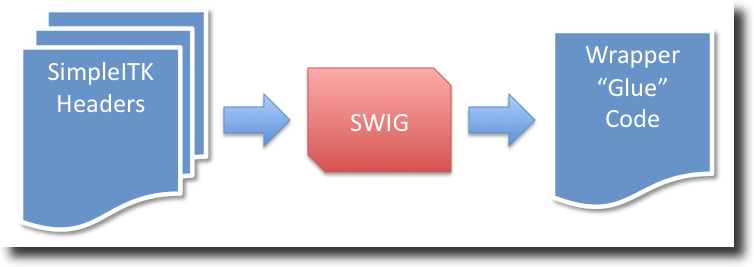
\includegraphics[width=.8\textwidth]{Images/WrappingProcess_shadow}
\end{center}
\begin{itemize}
  \item SimpleITK headers are constructed for wrapping
  \item SWIG is an open source package
  \begin{itemize}
    \item Parses C/C++ code, produces ``glue'' code
    \item Well supported, covers 10+ languages
  \end{itemize}
  \item Main languages: Python, Java, C\#
  \item Also supported: Tcl, Lua, R
\end{itemize}
\end{frame}

\begin{frame}[fragile]
\frametitle{Object Paradigm (Python)}
The paradigms translate to the wrapped languages (C++ $\rightarrow$ Python)
\lstcpp
\begin{lstlisting}
#include <SimpleITK.h>
using itk::simple;
...
// Create a smoothing filter
SmoothingRecursiveGaussianImageFilter gaussian;
// Set a parameter
gaussian.SetSigma ( 2.0 );
// "Execute" the Filter
Image blurredImage = gaussian.Execute ( image );
\end{lstlisting}
\lstpython
\begin{lstlisting}
from SimpleITK import *
# Create a smoothing filter
SmoothingRecursiveGaussianImageFilter gaussian
# Set a parameter
gaussian.SetSigma ( 2.0 );
# "Execute" the Filter
blurredImage = gaussian.Execute ( image );
\end{lstlisting}
\end{frame}

\begin{frame}[fragile]
\frametitle{Object Paradigm (Java)}
\lstjava
\begin{lstlisting}
import SimpleITK.*;
...

// Create a smoothing filter
SmoothingRecursiveGaussianImageFilter gaussian =
      new SmoothingRecursiveGaussianImageFilter();

// Set a parameter
gaussian.SetSigma ( 2.0 );

// "Execute" the Filter
Image blurredImage = gaussian.Execute ( image );
\end{lstlisting}
\end{frame}


\begin{frame}[fragile]
\frametitle{Object Paradigm (C\#)}
\lstjava
\begin{lstlisting}
using System;
using itk.simple;
...
// Create a smoothing filter
SmoothingRecursiveGaussianImageFilter gaussian =
      new SmoothingRecursiveGaussianImageFilter();

// Set a parameter
gaussian.SetSigma ( 2.0 );

// "Execute" the Filter
Image blurredImage = gaussian.Execute ( image );
\end{lstlisting}
\end{frame}


\begin{frame}{Note on the Tutorial}
\begin{itemize}
  \item Most examples will be Python
  \item Obvious translation to other languages
  \item C++ usage (generally) obvious
\end{itemize}
\end{frame}

\subsection{Example}
\begin{frame}{Hands On}
\fontsize{36pt}{36pt}\selectfont
\center
\begin{center}
Hands On
\end{center}
\end{frame}

\begin{frame}[fragile]
\frametitle{What just happened?}
\lstpython
\begin{lstlisting}
# Simple smoothing
smooth = SimpleITK.SmoothingRecursiveGaussian ( image, 2.0 )
SimpleITK.Show ( SimpleITK.Subtract ( image, smooth ) )
...
RuntimeError: Exception thrown in SimpleITK Subtract: ...
sitk::ERROR: Both images for SubtractImageFilter don't match type or dimension!
...
\end{lstlisting}

\begin{itemize}
  \item The output of SmoothingRecursiveGaussian is of type float
  \item The input image is signed short
  \item Most SimpleITK filters with 2 inputs require the same type
  \item Let's fix the problem
\end{itemize}

\end{frame}

\begin{frame}[fragile]
\frametitle{Introducing Cast}
\lstpython
\begin{lstlisting}
# Much better
smooth = SimpleITK.Cast ( smooth, image.GetPixelIDValue() )
print image.GetPixelIDTypeAsString()
print smooth.GetPixelIDTypeAsString()
SimpleITK.Show ( SimpleITK.Subtract ( image, smooth ) )
\end{lstlisting}
\end{frame}

%% Morphology
\subsection{Morphology}

\begin{frame}{Morphology}
\fontsize{36pt}{36pt}\selectfont
\center
\begin{center}
Morphology
\end{center}
\end{frame}

\begin{frame}[fragile]
\frametitle{Operators}

\begin{columns}[c]

\column{0.25\textwidth}
\begin{center}
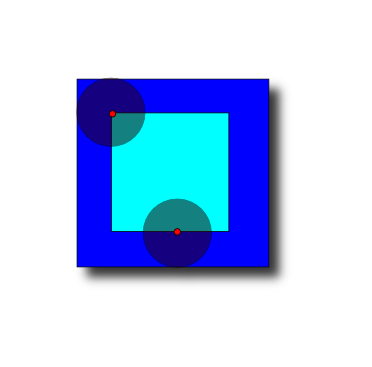
\includegraphics[width=1\textwidth]{Images/Erosion_shadow} \\
Erosion
\end{center}

\column{0.25\textwidth}
\begin{center}
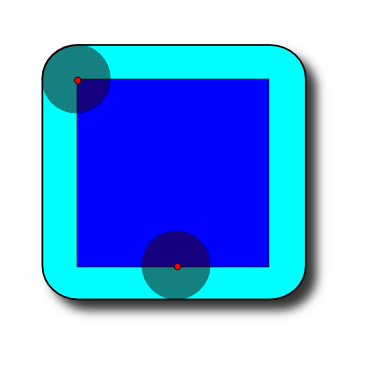
\includegraphics[width=1\textwidth]{Images/Dilation_shadow} \\
Dilation
\end{center}

\column{0.25\textwidth}
\begin{center}
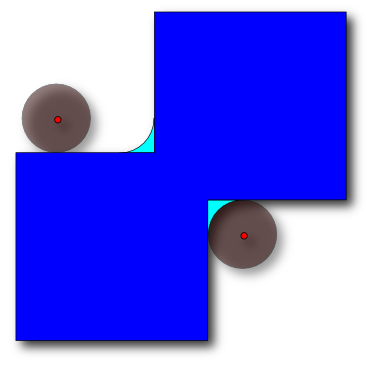
\includegraphics[width=1\textwidth]{Images/Closing_shadow} \\
Closing
\end{center}

\column{0.25\textwidth}
\begin{center}
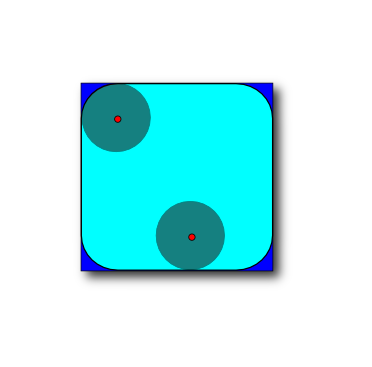
\includegraphics[width=1\textwidth]{Images/Opening_shadow} \\
Opening
\end{center}
\end{columns}
\vspace{12pt}
Images from \url{http://en.wikipedia.org/wiki/Mathematical_morphology}
\end{frame}

\begin{frame}{Morphology in Action}
\center
\begin{center}
Back to iPython
\end{center}
\end{frame}


\subsection{Label Maps}

%% Label maps
\begin{frame}{Label Maps}
\fontsize{36pt}{36pt}\selectfont
\center
\begin{center}
Label Maps
\end{center}
\end{frame}

%% Break
\begin{frame}{Break}
\fontsize{36pt}{36pt}\selectfont
\center
\begin{center}
Let's take a break
\end{center}
\end{frame}

